

\section{Accounting for Alternatives Chosen by the Control Group} \label{appendix:cbaresultscont}

\noindent Our main analysis so far compares the treatment to the control group, irrespective of the choice of childcare chosen by the families of the control-group children. This exercise compares treatment to the ``next best'' alternative that the parents of the control-group children elected. As we document in Section~\ref{section:background} of this paper, almost 75\% of the control-group children were enrolled in an alternative.

\noindent In this Appendix we disaggregate our estimates by computing social efficiency measures for ABC/CARE relative to (a) alternative (low-quality) formal childcare options and (b) staying at home. We refine our analysis to draw two further comparisons: (i) ABC/CARE compared to no treatment at all (so that the control child stayed at home); and (ii) ABC/CARE compared alternative preschool arrangements, which we describe in Section~\ref{section:background}.\footnote{\cite{Garcia_Heckman_Ziff_2018_EER} discuss this issue in depth.}

\noindent All treatment-group children have the same exposure. We simplify the analysis of the controls by creating two categories. ``$H$'' indicates that the control-group child is in home care throughout the entire length of the program. ``$C$'' indicates that a control-group child is in alternative center childcare for any amount of time.\footnote{In a companion paper, \cite{Garcia_Heckman_Ziff_2018_EER}, we show that this assumption is innocuous.} We thus compress a complex reality into two counterfactual outcome states at age $a$ for control-group subjects:
\begin{align*}
\bm{Y}_{a,H}^0 \quad &: \quad \textbf{ Subject received home care exclusively} \\
\bm{Y}_{a,C}^0 \quad &: \quad \textbf{ Subject received some alternative childcare}.
\end{align*}

\noindent We define $V$ as a dummy variable indicating participation by control-group children in an alternative childcare. $V=0$ denotes staying at home. The outcome when a child is in control status is
\begin{equation}
\bm{Y}^0_a : = \left( 1 - V \right) \bm{Y}^0_{a,H} + \left( V \right) \bm{Y}^0_{a,C}. \label{eq:meandiff}
\end{equation}

\noindent It is fruitful to assess the effectiveness of the program with respect to a counterfactual world in which the child stays at home full time. The associated causal parameter for those who would choose to keep the child at home is:
\begin{equation}\label{eq:influenza}
\bm{\Delta}_a \left(\text{\textbf{Fix }} V = 0 \right) :=   \mathbb{E} \left[ \bm{Y}^1_a - \bm{Y}^0_a | \text{\textbf{Fix }} V = 0, W = 1 \right] = \mathbb{E} \left[\bm{Y}^1_{a} - \bm{Y}^0_{a,H} | \text{\textbf{Fix }} V = 0, \bm{B} \in \mathcal{B}_0 \right].
\end{equation}
where $\text{\textbf{Fix }} V$ refers to fixing $V$ rather than just conditioning on it.\footnote{For the distinction between fixing and conditioning, see \cite{Heckman_Pinto_2015_EconometTheory}.}

\noindent It is also useful to assess the effectiveness of a program relative to attendance in an alternative childcare center for those who would choose an alternative:

\begin{equation}\label{eq:smallpox}
\bm{\Delta}_a \left(\text{\textbf{Fix }} V =1 \right) :=   \mathbb{E} \left[ \bm{Y}^1_a - \bm{Y}^0_a | \text{\textbf{Fix }} V = 1, W = 1 \right] = \mathbb{E} \left[\bm{Y}^1_a - \bm{Y}^0_{a,C} | \text{\textbf{Fix }} V = 1, \bm{B} \in \mathcal{B}_0 \right].
\end{equation}

\noindent Random assignment to treatment does not directly identify \eqref{eq:influenza} or \eqref{eq:smallpox}. Econometric methods are required to identify these parameters. In this paper we rely on matching (conditioning on observables) to control for selection into the home or take-up of alternatives. In \cite{Garcia_Heckman_Ziff_2018_EER}, we document that alternative approaches to selection produce similar estimates. We combine the matching strategies with the methodology in Section~\ref{section:cbamethodology} to produce forecasts and provide measures of social efficiency refining the counterfactual comparison for the control-group children.

\noindent Figure~\ref{fig:npvsgender} summarizes our estimates. There are substantial differences between males and females in one counterfactual: treatment vs. alternative preschools. The estimated treatment effects are very similar across genders for treatment compared to those staying at home full time. Males benefit much more from treatment relative to alternative preschools compared to their benefits from treatment relative to staying at home. This result is consistent with findings noted elsewhere: (i) fathers are more likely to remain at home with the mother if the child is a boy and such families have more resources, diminishing the treatment effect for ABC/CARE compared to the home alternative, and (ii) boys are more adversely affected by low quality formal childcare environments. The formal alternative childcare centers are of generally low quality (see \citealp{Garcia_Heckman_Ziff_2018_EER}).

\noindent For females, there is a gain of 4.93 dollars per dollar invested compared to staying at home. When we decompose the net-present value for each of the components that we monetize, we find substantial benefits for females across a variety of categories, including health and crime. For males, the magnitudes are noticeably increased when comparing outcomes from treatment to outcomes from attending alternative preschools.

\begin{sidewaysfigure}[!htbp]
\centering
\caption{Life-cycle Net Present Value of Main Components of the CBA}\label{fig:npvsgender}
\begin{subfigure}[h]{0.5\textwidth}
		\centering
		\caption{Males}
		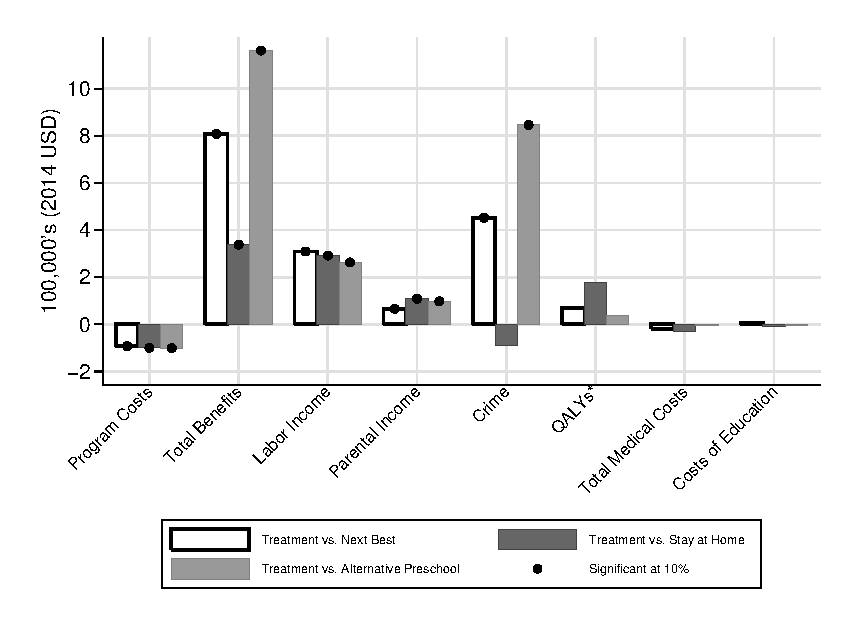
\includegraphics[width=\textwidth]{output/abccare_npvs2.eps}
\end{subfigure}%
\begin{subfigure}[h]{0.5\textwidth}
		\centering
		\caption{Females}
		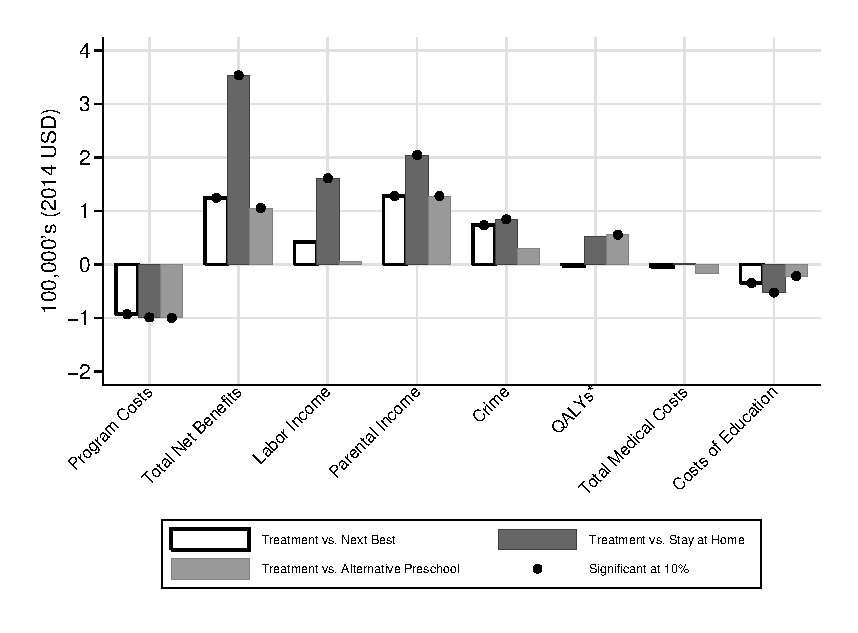
\includegraphics[width=\textwidth]{output/abccare_npvs1.eps}
\end{subfigure}
\footnotesize \justify
Note: This figure displays the life-cycle net present values of the main components of the cost/benefit analysis of ABC/CARE from birth to forecasted death, discounted to birth at a rate of 3\%. ``Treatment vs. Next Best'': compares the treatment to the control group. ``Treatment vs. Stay at Home'': compares the treatment group to those subjects who stayed at home. ``Treatment vs. Alternative Preschool'': compares the treatment group to those subjects who attended alternative preschools. The latter two are based on matching estimators that account for selection on observable variables. By ``net" we mean that each component represents the total value for the treatment group minus the total value for the control group. Program costs: the total cost of ABC/CARE, including the welfare cost of taxes to finance it. Total net benefits: are for \textit{all} of the components we consider. Labor income: total individual labor income from ages 20 to the retirement of program participants (assumed to be age 67). Parental labor income: total parental labor income of the parents of the participants from when the participants were ages 1.5 to 21. Crime: the total cost of crime (judicial and victimization costs). To simplify the display, the following components are not shown in the figure: (i) cost of alternative preschool paid by the parents of control group children; (ii) the social welfare costs of transfer income from the government; (iii) disability benefits and social security claims; (iv) costs of increased individual and maternal education (including special education and grade retention); (v) total medical public and private costs. Inference is based on non-parametric, one-sided $p$-values from the empirical bootstrap distribution. We indicate point estimates significant at the $10\%$ level.\\
*The treatment vs. stay at home net present value is sizable and negative (-\$123,498.2); its standard error is \$62,745.72.\\
**QALYs refers to the quality-adjusted life years. Any gain corresponds to better health conditions until forecasted death, with $\$150,000$ (2014 USD) as the base value for a year of life.
\end{sidewaysfigure} 